\section{Results}
In this section, we present the results obtained from our sentiment analysis models applied to tweet data. We detail the different approaches and techniques used, focusing on the models that demonstrated effective performance in classifying tweet sentiment.

Initially, we explored traditional Machine Learning (ML) models, such as Support Vector Machines (SVMs), utilizing both Bag-of-Words (BoW) and TF-IDF features for text representation. This established a foundational understanding of model performance on our dataset. Concurrently, we investigated lexicon-based approaches, specifically VADER and TextBlob, to leverage pre-defined sentiment scores.

Subsequently, we delved into various neural network architectures. This included Feedforward Neural Networks (FNNs), Convolutional Neural Networks (CNNs) adapted for text classification, and several Recurrent Neural Networks (RNNs). Within RNNs, we experimented with Long Short-Term Memory (LSTM) networks, Gated Recurrent Units (GRU), and Bidirectional LSTMs (Bi-LSTMs).

Finally, we implemented the powerful transformer-based model, BERT, a state-of-the-art architecture known for its strong performance in natural language processing tasks. Our analysis focused on BERT's ability to accurately classify tweet sentiment.

\subsection{Machine Learning models}

We began our exploration of sentiment analysis by employing traditional Machine Learning (ML) models, specifically Support Vector Machines (SVMs). These models serve as a robust baseline, leveraging established techniques for text classification. To convert raw tweet content into a format understandable by these algorithms, we utilized two distinct feature representation methods: Bag-of-Words (BoW) and TF-IDF (Term Frequency-Inverse Document Frequency). For each SVM variant, we performed meticulous hyperparameter tuning to optimize its performance, ensuring the models were finely tuned for our dataset.

For the hyperparameter optimization of both SVM models, we utilized RandomizedSearchCV. The range of parameters explored and the search configuration are detailed in the table below:

\begin{table}[H]
\centering
\caption{Hyperparameter Tuning Configuration for SVM Models}
\begin{tabular}{|l|l|}
\hline
\multicolumn{2}{|c|}{\textit{SVM Hyperparameters}} \\
\hline
\textbf{Parameter} & \textbf{Values Explored} \\
\hline
C & [0.01, 0.1, 1, 10] \\
kernel & ['linear', 'rbf'] \\
gamma & ['scale', 'auto'] \\
\hline\hline 
\multicolumn{2}{|c|}{\textit{RandomizedSearchCV Settings}} \\
\hline
n\_iter & 5 (number of parameter settings sampled) \\
cv & 3 (number of cross-validation folds) \\
\hline
\end{tabular}
\label{tab:svm_tuning_params}
\end{table}



\subsubsection{\textbf{Support Vector Machines (SVMs) with TF-IDF}}

Our initial SVM approach utilized the TF-IDF Vectorizer to transform the processed tweet texts into numerical features. This method is highly effective for text classification as it weighs words by their frequency within a document, inversely scaled by their frequency across the entire corpus. This approach assigns higher importance to terms that are distinctive to a particular tweet while being less common overall, thus capturing valuable information. The TF-IDF Vectorizer was configured with max\_features=10000, ngram\_range=(1, 2) (allowing for both single words and two-word phrases), min\_df=2 (excluding terms appearing in fewer than two documents), max\_df=0.8 (excluding terms appearing in more than 80\% of documents to remove common words), and incorporated English stop words removal.

Based on the RandomizedSearchCV process, the best parameters identified for the SVM with TF-IDF were 
\begin{itemize}
    \item 'kernel': 'rbf'
    \item 'gamma': 'scale'
    \item 'C': 10
\end{itemize}

The performance of the SVM model with TF-IDF features on the test set is detailed below:

\begin{table}[H]
\centering
\caption{Classification Report for SVM with TF-IDF}
\begin{tabular}{|l|c|c|c|c|}
\hline
\textbf{Class} & \textbf{Precision} & \textbf{Recall} & \textbf{F1-Score} & \textbf{Support} \\
\hline
positive & 0.94 & 0.93 & 0.94 & 4287 \\
negative & 0.94 & 0.92 & 0.93 & 3465 \\
neutral  & 0.90 & 0.94 & 0.92 & 3869 \\
\hline
\textbf{Accuracy} & \multicolumn{4}{|c|}{\textbf{0.93}} \\
\hline
\end{tabular}
\label{tab:svm_tfidf_report}
\end{table}

The SVM with TF-IDF achieved an overall accuracy of 0.93 on the test set, indicating its strong capability in classifying tweet sentiment. The model demonstrated robust performance across all sentiment categories, achieving notably high precision and recall, particularly for the 'positive' class. The F1-scores further underscore a good balance between precision and recall for all classes, confirming the model's effectiveness.

\subsubsection{\textbf{Support Vector Machines (SVMs) with Bag-of-Words}}

We also implemented an SVM model using the Bag-of-Words (BoW) approach with CountVectorizer for text representation. This method converts text into a numerical format by simply counting the occurrences of each word, providing a frequency-based representation of the tweet content. The CountVectorizer was configured with the same parameters as the TF-IDF Vectorizer: max\_features=10000, ngram\_range=(1, 2), min\_df=2, max\_df=0.8, and English stop words removal.

Following the same RandomizedSearchCV process as detailed in Table \ref{tab:svm_tuning_params}, the optimal hyperparameters identified for the SVM with Bag-of-Words were also:
\begin{itemize}
    \item 'kernel': 'rbf'
    \item 'gamma': 'scale'
    \item 'C': 10
\end{itemize}

The model's performance on the test data is detailed in the following table:

\begin{table}[H]
\centering
\caption{Classification Report for SVM with Bag-of-Words}
\begin{tabular}{|l|c|c|c|c|}
\hline
\textbf{Class} & \textbf{Precision} & \textbf{Recall} & \textbf{F1-Score} & \textbf{Support} \\
\hline
positive & 0.92 & 0.91 & 0.91 & 4287 \\
negative & 0.92 & 0.88 & 0.90 & 3465 \\
neutral  & 0.87 & 0.91 & 0.89 & 3869 \\
\hline
\textbf{Accuracy} & \multicolumn{4}{|c|}{\textbf{0.90}} \\
\hline
\end{tabular}
\label{tab:svm_bow_report}
\end{table}


The SVM with Bag-of-Words achieved an accuracy of 0.90, which was slightly lower than the accuracy attained by its TF-IDF counterpart. While still performing well across sentiment classes, particularly for the 'positive' category, the marginal difference in overall accuracy and F1-scores suggests that the TF-IDF representation had a slight advantage in capturing the nuanced importance of words in the dataset.

\subsubsection{\textbf{Comparative Analysis of SVM Models}}

Figure \ref{fig:svm_comparison} provides a visual comparison of the accuracies and confusion matrices for both SVM models, offering a clear overview of their respective performances.

\begin{figure}[h!]
\centering
\begin{subfigure}[t]{0.30\textwidth}
\centering
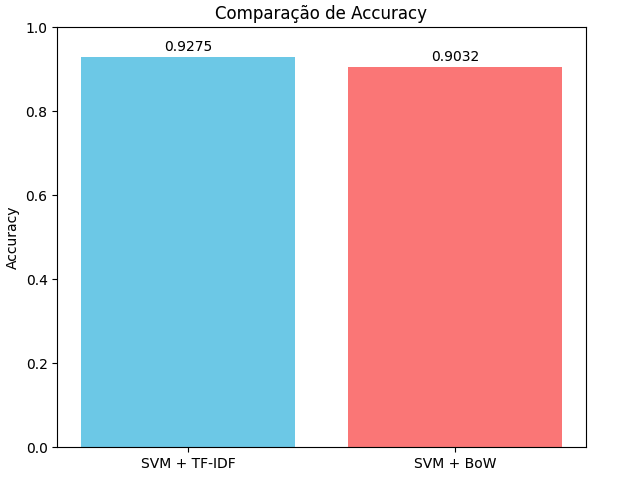
\includegraphics[width=\textwidth]{./images/svm_accuracies.png}
\caption{Accuracy Comparison: SVM + TF-IDF vs. SVM + BoW}
\label{fig:svm_accuracies}
\end{subfigure}
\hfill
\begin{subfigure}[t]{0.30\textwidth}
\centering
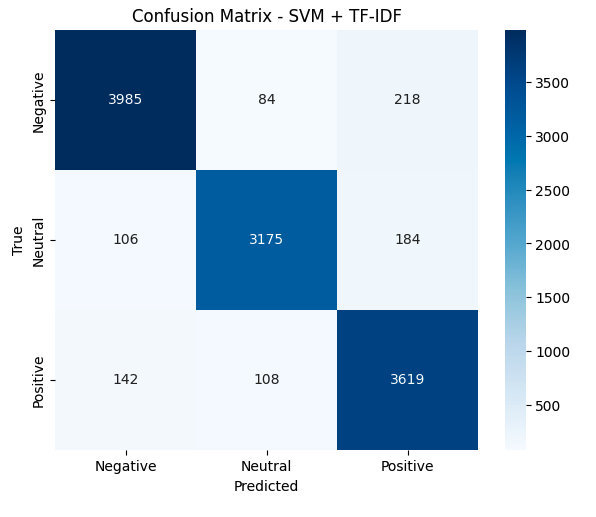
\includegraphics[width=\textwidth]{./images/cm-svm-tfidf.png}
\caption{Confusion Matrix - SVM + TF-IDF}
\label{fig:cm_tfidf}
\end{subfigure}
\hfill
\begin{subfigure}[t]{0.30\textwidth}
\centering
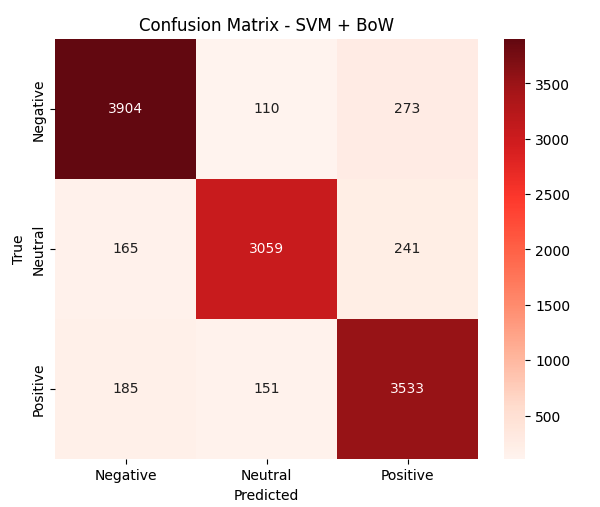
\includegraphics[width=\textwidth]{./images/cm-svm-bow.png}
\caption{Confusion Matrix - SVM + BoW}
\label{fig:cm_bow}
\end{subfigure}
\caption{Performance Comparison of SVM Models}
\label{fig:svm_comparison}
\end{figure}

The comparative accuracy bar chart clearly illustrates that TF-IDF features generally yielded superior performance for SVM in this sentiment classification task. The confusion matrices offer a detailed view of the models' classification strengths and weaknesses across the different sentiment classes. Both models exhibited a tendency to misclassify some 'neutral' tweets, which often present greater ambiguity in sentiment compared to clearly 'positive' or 'negative' content. However, we can see in the confusion matrix that TF-IDF model indicates slightly better classification rates across all categories.

These traditional ML models establish a solid baseline for our sentiment analysis efforts, demonstrating the effectiveness of classic text representation techniques when paired with a powerful classifier like SVM. Their performance underscores the enduring importance of careful feature engineering in achieving robust machine learning outcomes.




\subsection{ Traditional approaches}

Beyond machine learning models, we explored lexicon-based approaches for sentiment analysis. These methods rely on predefined dictionaries of words, each associated with a sentiment score. We specifically utilized TextBlob and VADER (Valence Aware Dictionary and sEntiment Reasoner),


\subsubsection{ \textbf{TextBlob Sentiment Analysis}}

TextBlob is a Python library for processing textual data, providing a simple API for common natural language processing (NLP) tasks, including sentiment analysis. Its sentiment analysis model returns two properties: polarity (a float ranging from -1.0 to 1.0, where -1 is negative, 0 is neutral, and 1 is positive) and subjectivity (a float ranging from 0.0 to 1.0, where 0.0 is very objective and 1.0 is very subjective).

For sentiment classification, we defined a rule-based approach:
\begin{itemize}
    \item Polarity greater than 0.1 was classified as 'Positive'.
    \item Polarity less than -0.1 was classified as 'Negative'.
    \item Polarity between -0.1 and 0.1 (inclusive) was classified as 'Neutral'.
\end{itemize}

The performance of TextBlob on the validation dataset, using this classification logic, is summarized below:

\begin{table}[H]
\centering
\caption{Classification Report for TextBlob (Validation Set)}
\begin{tabular}{|l|c|c|c|c|}
\hline
\textbf{Class} & \textbf{Precision} & \textbf{Recall} & \textbf{F1-Score} & \textbf{Support} \\
\hline
Negative & 0.53 & 0.44 & 0.48 & 266 \\
Neutral  & 0.39 & 0.39 & 0.39 & 285 \\
Positive & 0.53 & 0.61 & 0.57 & 276 \\
\hline
\textbf{Accuracy} & \multicolumn{4}{|c|}{\textbf{0.48}} \\
\hline
\end{tabular}
\label{tab:textblob_validation_report}
\end{table}

TextBlob achieved an accuracy of 0.48 on the validation set. While it performed reasonably well for 'Positive' sentiment, its ability to correctly identify 'Neutral' and 'Negative' tweets was limited, as indicated by lower precision and recall scores for those categories. This suggests that its lexicon-based rules might struggle with the nuances and informal language often found in tweets.

\begin{figure}[H]
    \centering
    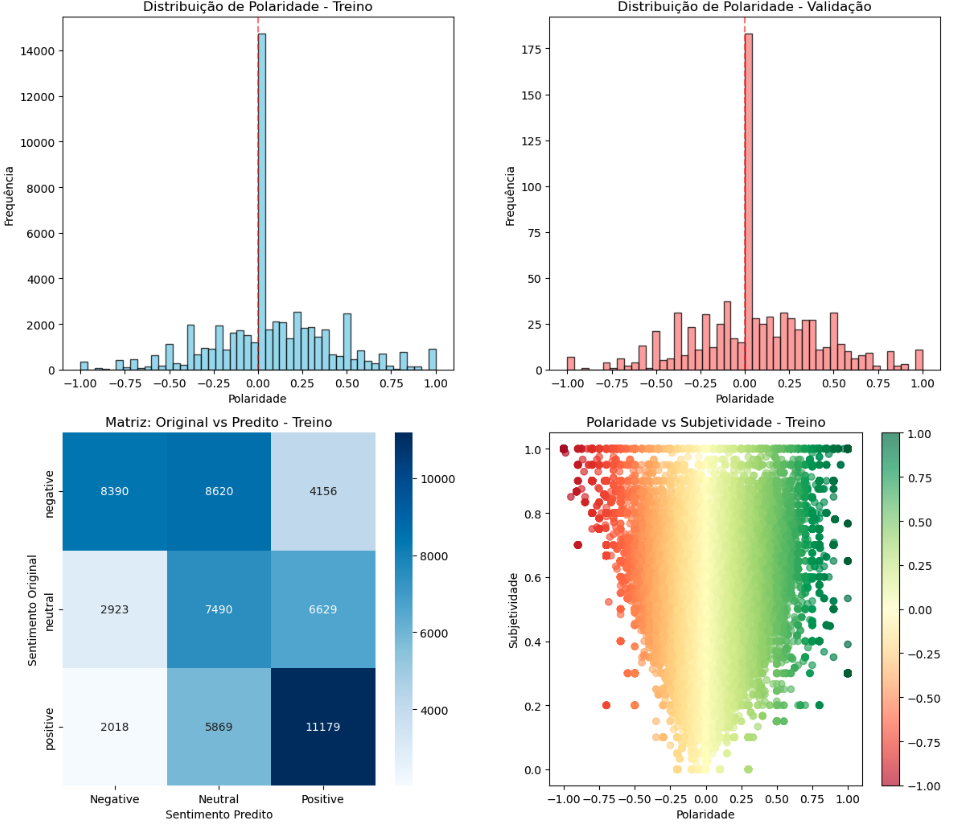
\includegraphics[width=1\linewidth]{images/text-blob.png}
    \caption{Correlation Matrix and Polarity Distribution}
    \label{fig:enter-label}
\end{figure}

The polarity distributions show a concentration of scores around zero, indicating many tweets are classified as neutral. The confusion matrix highlights challenges in distinguishing between sentiment classes, particularly the 'Neutral' class, which is often misclassified.


\subsubsection{ \textbf{VADER Sentiment Analysis}}
VADER (Valence Aware Dictionary and sEntiment Reasoner) is a lexicon and rule-based sentiment analysis tool specifically attuned to sentiments expressed in social media contexts. Unlike TextBlob's polarity, VADER provides a compound score (normalized between -1 and 1) representing the overall sentiment intensity, along with positive, negative, and neutral scores. Its strength lies in recognizing common linguistic features of internet language, such as capitalization, exclamation marks, and emojis, which significantly influence sentiment.

For classification, we used VADER's compound score with a standard threshold:
\begin{itemize}
    \item Compound score >= 0.05: 'Positive'
    \item Compound score <= -0.05: 'Negative'
    \item Compound score between -0.05 and 0.05: 'Neutral'
\end{itemize}

The performance of VADER on the validation dataset is presented below:

\begin{table}[H]
\centering
\caption{Classification Report for VADER (Training Set)}
\begin{tabular}{|l|c|c|c|c|}
\hline
\textbf{Class} & \textbf{Precision} & \textbf{Recall} & \textbf{F1-Score} & \textbf{Support} \\
\hline
Negative & 0.56 & 0.58 & 0.57 & 21166 \\
Neutral  & 0.34 & 0.18 & 0.24 & 17042 \\
Positive & 0.50 & 0.68 & 0.57 & 19066 \\
\hline
\textbf{Accuracy} & \multicolumn{4}{|c|}{\textbf{0.50}} \\
\hline
\end{tabular}
\label{tab:vader_training_report}
\end{table}


VADER outperformed TextBlob, achieving an accuracy of 0.50 on the validation set. Its higher precision, recall, and F1-scores across all classes, especially for 'Negative' and 'Positive' sentiments, highlight its effectiveness in handling the specific characteristics of social media text. The 'Neutral' class still presented some challenges, but VADER's performance was better than TextBlob.

Figure \ref{fig:vader_analysis} provides a visual representation of VADER's sentiment scores and classifications:

\begin{figure}[H]
    \centering
    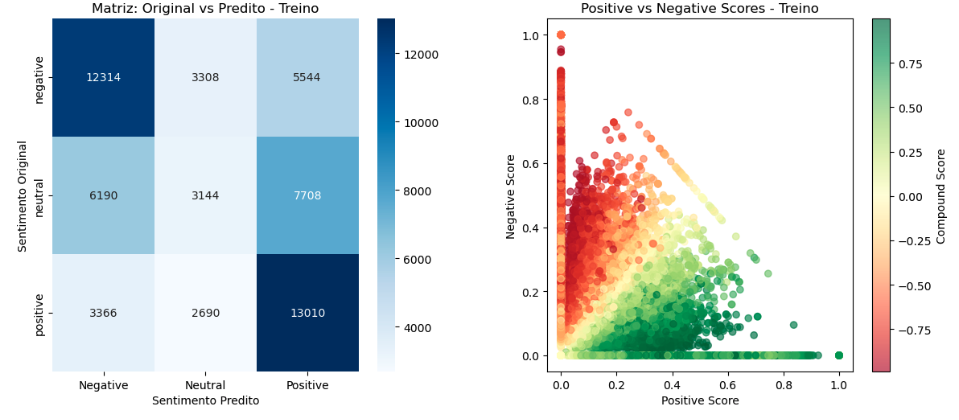
\includegraphics[width=1\linewidth]{images/vader.png}
    \caption{Correlation Matrix, Positive vs Negative}
    \label{fig:vader_analysis}
\end{figure}

The compound score distributions show a clearer separation of positive and negative sentiments compared to TextBlob. The confusion matrix further demonstrates VADER's improved classification abilities, but the neutral class still has problems.


\subsubsection{\textbf{Comparative Analysis}}

Comparing TextBlob and VADER, it's clear that VADER provides a more robust and accurate sentiment analysis for tweets among the lexicon-based methods. 

However, when comparing these traditional lexicon-based approaches to the Machine Learning models (SVMs) previously discussed, it is evident that the SVMs achieved significantly higher overall accuracies.  These results demonstrate that while lexicon-based models offer fast and lightweight sentiment scoring without explicit training, their performance is generally surpassed by supervised machine learning models that can learn complex patterns directly from the labeled data. This difference highlights the benefit of data-driven learning in capturing intricate semantic and contextual relationships, which static lexicons may struggle to interpret.



\subsection{Deep Learning Models}

After explored traditional machine learning and lexicon-based approaches, we explore into Deep Learning (DL) models to leverage their capability in learning complex patterns directly from raw data. This section details our experiments with Feedforward Neural Networks (FNNs), Convolutional Neural Networks (CNNs) adapted for text, Recurrent Neural Networks (RNNs), and the transformer-based BERT model.

\subsubsection{\textbf{Feedforward Neural Networks (FNNs)}}

Our initial deep learning experiments began with Feedforward Neural Networks (FNNs). These models consist of multiple layers where information flows in one direction, from input to output, without cycles. FNNs are a foundational architecture for learning complex, non-linear relationships. We integrated an Embedding layer as the first component, which maps words to dense vector representations, allowing the model to capture semantic similarities between words. We explored two main configurations for our FNNs:

\textbf{First FNN Architecture
}

The first FNN architecture used a straightforward approach to flatten the output of the embedding layer before feeding it into dense layers. This creates a single, long feature vector from the word embeddings.

The model's architecture is as follows:

\begin{itemize}
    \item Embedding Layer: Maps vocabulary words to 100-dimensional dense vectors.
    \item Flatten Layer: Converts the 2D output of the embedding layer into a 1D vector.
    \item Dense Layer (128 units): Fully connected layer with ReLU activation.
    \item Dropout Layer (0.5): Regularization to prevent overfitting by randomly setting 50\% of input units to 0.
    \item Dense Layer (64 units): Another fully connected layer with ReLU activation.
    \item Dropout Layer (0.3): Regularization, setting 30\% of input units to 0.
    \item Output Layer (3 units): Dense layer with Softmax activation for multiclass classification (positive, neutral, negative).
\end{itemize}

The model was compiled using the Adam optimizer with a learning rate of 0.001 and categorical crossentropy as the loss function.

\textbf{Second FNN Architecture}

The second FNN architecture aimed to improve upon the first by replacing the Flatten layer with GlobalAveragePooling1D and incorporating BatchNormalization and L2 regularization into the dense layers. GlobalAveragePooling1D reduces the dimensionality by averaging embedding vectors across the sequence length, preserving more semantic information than flattening. BatchNormalization helps stabilize and accelerate training, while L2 regularization penalizes large weights, which can mitigate overfitting.

The model's architecture is as follows:

\begin{itemize}
    \item Embedding Layer: Maps vocabulary words to 100-dimensional dense vectors.
    \item GlobalAveragePooling1D Layer: Averages the word embeddings across the sequence.
    \item Dense Layer (128 units): Fully connected layer with ReLU activation and L2 regularization (0.01).
    \item BatchNormalization Layer: Normalizes the activations of the previous layer.
    \item Dropout Layer (0.5): Regularization.
    \item Dense Layer (64 units): Another fully connected layer with ReLU activation and L2 regularization (0.01).
    \item BatchNormalization Layer: Normalizes the activations.
    \item Dropout Layer (0.5): Regularization.
    \item Output Layer (3 units): Dense layer with Softmax activation.
    \item 
\end{itemize}
This model was also compiled using the Adam optimizer with a learning rate of 0.001, categorical crossentropy loss.

\textbf{Performance of FNN Models
}

Across both FNN architectures, while the models showed promising learning curves on the training data, they consistently exhibited signs of overfitting. The training accuracy would increase steadily, and the training loss would decrease, but the validation accuracy often plateaued or even declined after a few epochs, accompanied by an increase in validation loss. This indicates that the models were memorizing the training data rather than generalizing well to unseen examples. This behavior is a common challenge with FNNs on text data, as they may struggle to capture local features or sequences without more specialized architectures like CNNs or RNNs.

The subsequent figures illustrate this overfitting behavior:

\begin{figure}[h!]
\centering

% Primeira linha: FNN Architecture 1 Accuracy and Loss
\begin{subfigure}[t]{0.48\textwidth}
\centering
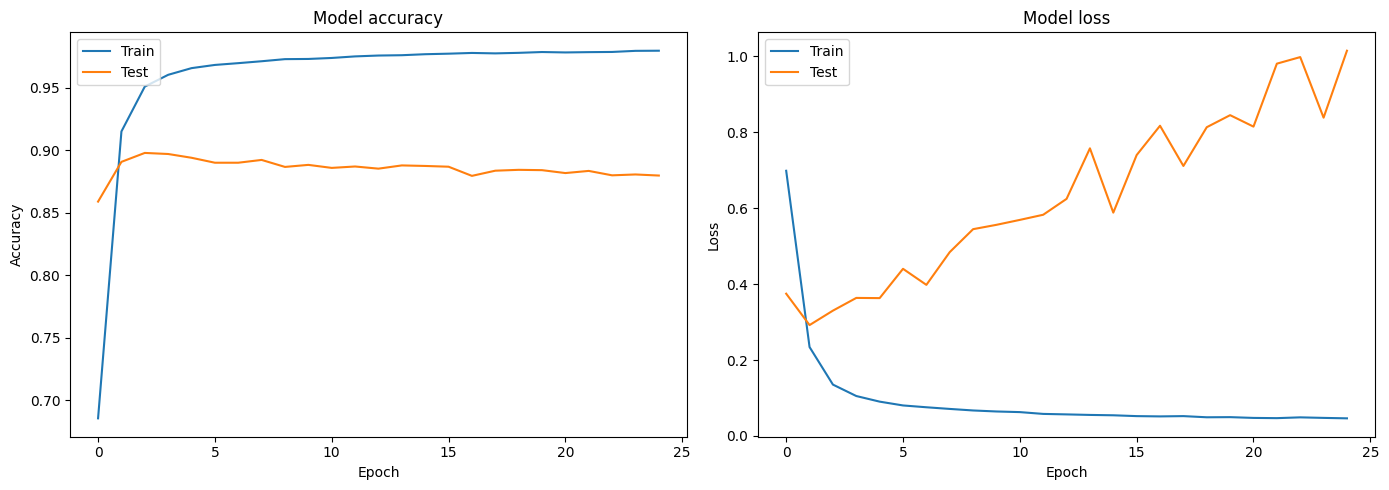
\includegraphics[width=\textwidth]{./images/fnn1-acc.png}
\caption{FNN Architecture 1: Train vs Validation Accuracy and Loss}
\label{fig:fnn1_accuracy}
\end{subfigure}

\vspace{0.5cm} % Espaçamento vertical entre as linhas

% Segunda linha: FNN Architecture 2 Accuracy and Loss
\begin{subfigure}[t]{0.48\textwidth}
\centering
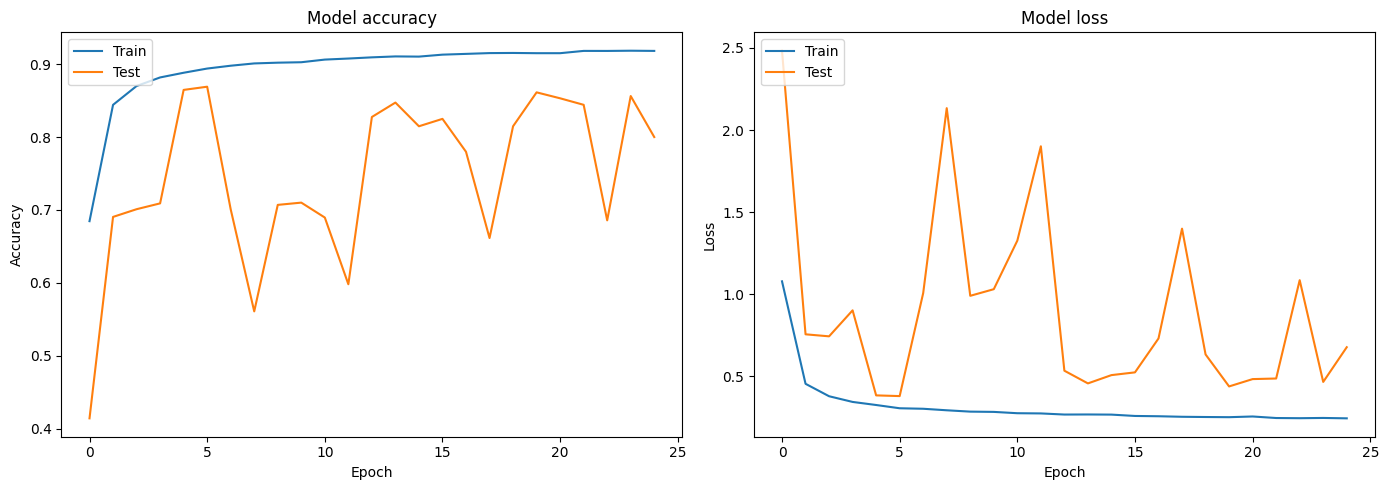
\includegraphics[width=\textwidth]{./images/fnn2-acc.png}
\caption{FNN Architecture 2: Train vs Validation Accuracy and Loss}
\label{fig:fnn1_loss}
\end{subfigure}

\vspace{0.5cm}

% Terceira linha: Confusion Matrices lado a lado
\begin{subfigure}[t]{0.23\textwidth}
\centering
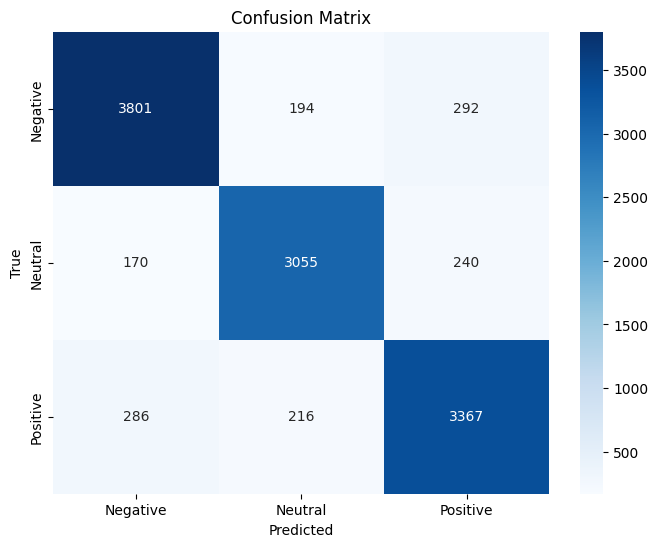
\includegraphics[width=\textwidth]{./images/fnn1-cm.png}
\caption{FNN Architecture 1: Confusion Matrix}
\label{fig:fnn2_accuracy}
\end{subfigure}
\hfill
\begin{subfigure}[t]{0.23\textwidth}
\centering
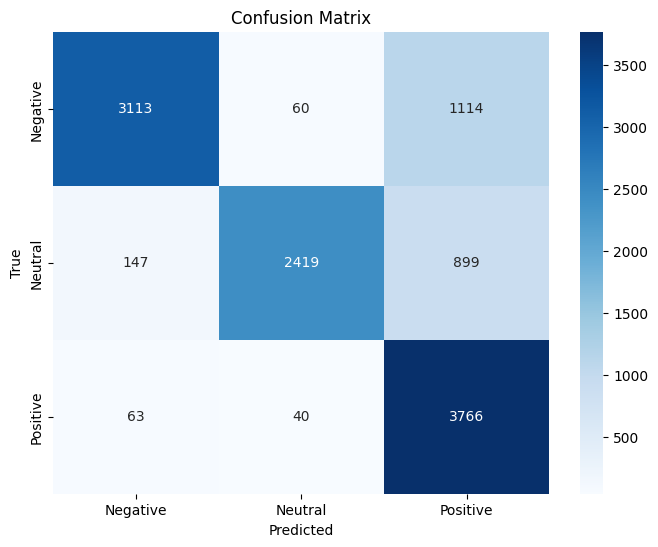
\includegraphics[width=\textwidth]{./images/fnn2-cm.png}
\caption{FNN Architecture 2: Confusion Matrix}
\label{fig:fnn2_loss}
\end{subfigure}
\caption{Training and Validation Performance of FNN Models}
\label{fig:fnn_performance}
\end{figure}

Given these limitations, particularly the persistent overfitting, we proceeded to explore more specialized deep learning architectures better suited for sequential data like text.

\subsubsection{\textbf{Convolutional Neural Networks (CNNs)}}

Following our experiments with FNNs, we moved on to Convolutional Neural Networks (CNNs). While traditionally known for image processing, CNNs have proven effective for text classification. They excel at capturing local patterns (like n-grams) through convolutional filters, regardless of their position in the sequence, and then aggregating these features.

We implemented two distinct CNN architectures:

\textbf{First CNN Architecture}

Our first CNN model utilized a single Conv1D layer followed by GlobalMaxPooling1D. This design aims to identify the most salient feature (the highest value detected by a filter) across the entire sequence for each filter.

The model's architecture is as follows:

\begin{itemize}
    \item Embedding Layer: Maps vocabulary words to 100-dimensional dense vectors (vocab\_size input dimension, maxlen input length).
    \item Conv1D Layer (128 filters): Applies 1D convolution with a kernel\_size of 5, using ReLU activation to detect local patterns.
    \item GlobalMaxPooling1D Layer: Extracts the maximum value from each feature map, effectively capturing the most important feature detected by each filter.
    \item Dense Layer (64 units): Fully connected layer with ReLU activation and L2 regularization (0.01).
    \item Dropout Layer (0.5): Regularization.
    \item Output Layer (3 units): Dense layer with Softmax activation for multiclass classification.
\end{itemize}

The model was compiled using the Adam optimizer with a learning rate of 0.001 and categorical crossentropy as the loss function.

\begin{figure}[h!]
    \centering
    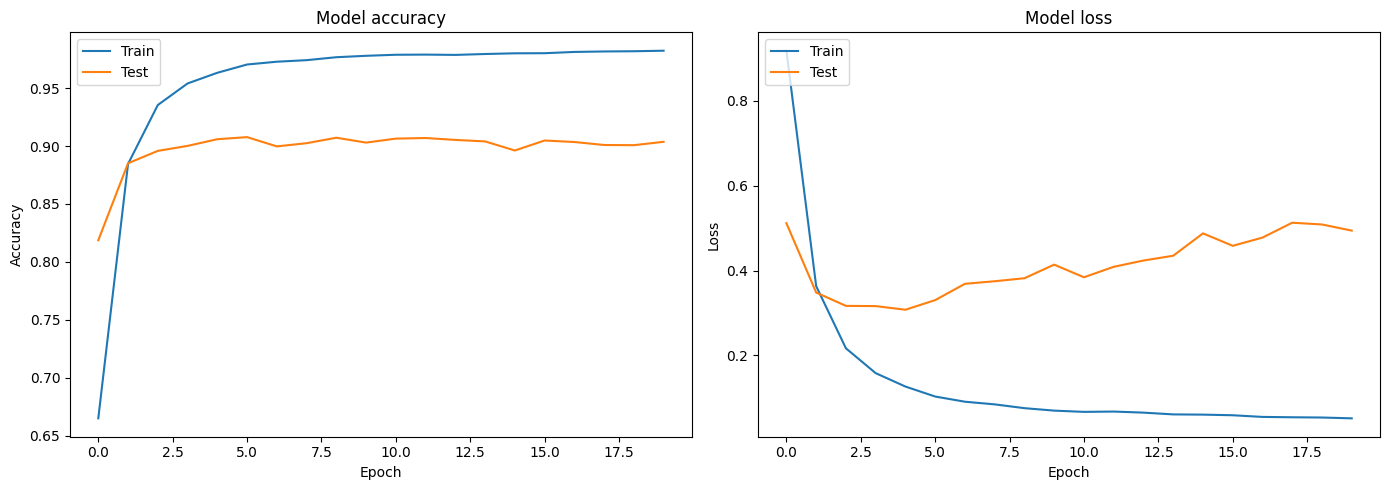
\includegraphics[width=1\linewidth]{images/cnn1-acc.png}
\caption{CNN Architecture 1: Train vs Validation Accuracy and Loss}
    \label{fig:cnn-acc-1}
\end{figure}

Similar to the FNNs, this first CNN architecture, despite its convolutional capabilities, still displayed significant overfitting. While it learned to classify the training data very well, its performance on the validation set would often diverge, indicating a struggle to generalize to new, unseen tweets. This suggests that a single-filter approach, even with regularization, might not be sufficient to capture the diverse patterns needed for robust sentiment classification on this dataset. The  figure \ref{fig:cnn-acc-1} illustrate the training and validation performance, clearly showing overfitting.

\textbf{Second CNN Architecture}

To address the limitations of the single-filter approach and improve generalization, our second CNN architecture adopted a multi-filter strategy, processing different n-gram sizes (3, 4, and 5) in parallel. This allows the model to extract a richer set of local features from the text, capturing patterns of varying lengths simultaneously. The outputs from these parallel filters are then concatenated and passed through a denser network.

The model's architecture is as follows:

\begin{itemize}
    \item Input Layer: Defines the input sequence length (maxlen).
    \item Embedding Layer: Maps vocabulary words to 100-dimensional dense vectors.
    \item Parallel Conv1D Layers (64 filters each):
     \begin{itemize}
 \item Conv1D with kernel\_size=3, ReLU activation, and L2 regularization (0.01).
     \item Conv1D with kernel\_size=4, ReLU activation, and L2 regularization (0.01).
     \item Conv1D with kernel\_size=5, ReLU activation, and L2 regularization (0.01).
     \end{itemize}
    \item Parallel GlobalMaxPooling1D Layers: Extracts the maximum feature from each of the three convolutional outputs.
    \item Concatenate Layer: Combines the outputs from the three pooling layers into a single vector.
    \item Dense Layer (32 units): Fully connected layer with ReLU activation and L2 regularization (0.05).
    \item Dropout Layer (0.6): Regularization.
    \item Output Layer (3 units): Dense layer with Softmax activation.
\end{itemize}

This model was compiled using the Adam optimizer with a learning rate of 0.001, categorical crossentropy loss.

\begin{figure}[h!]
\centering
\begin{subfigure}[t]{0.48\textwidth}
\centering
% Replace with your actual CNN 2 Accuracy plot
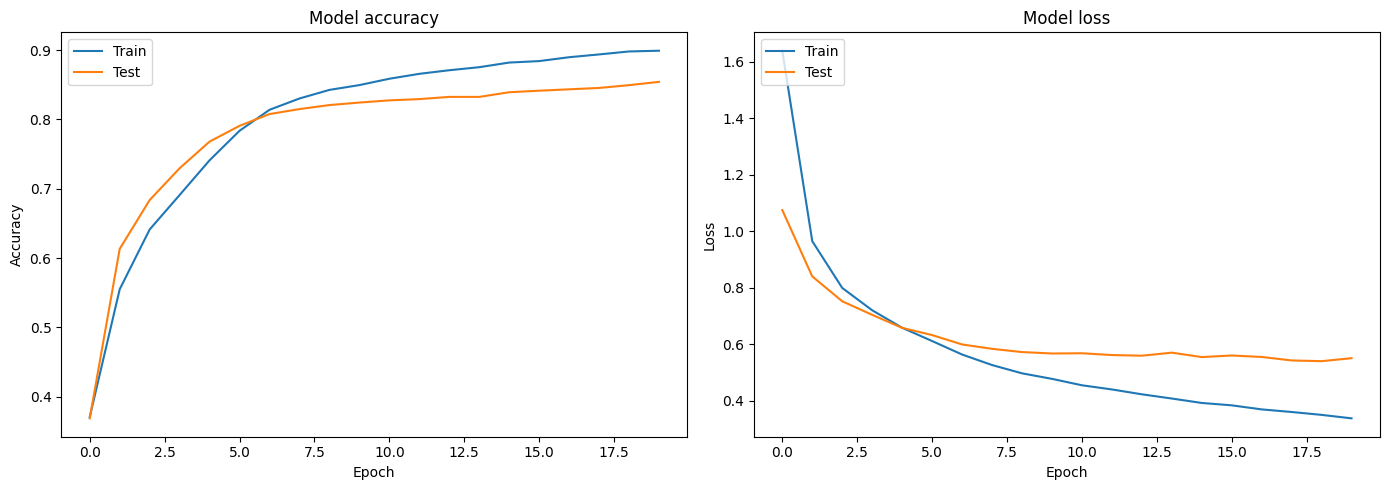
\includegraphics[width=\textwidth]{./images/cnn2-acc.png}
\caption{CNN Architecture 2: Train vs Validation Accuracy and Loss}
\label{fig:cnn2_accuracy}
\end{subfigure}
\hfill
\begin{subfigure}[t]{0.30\textwidth}
\centering
% Replace with your actual CNN 2 Loss plot
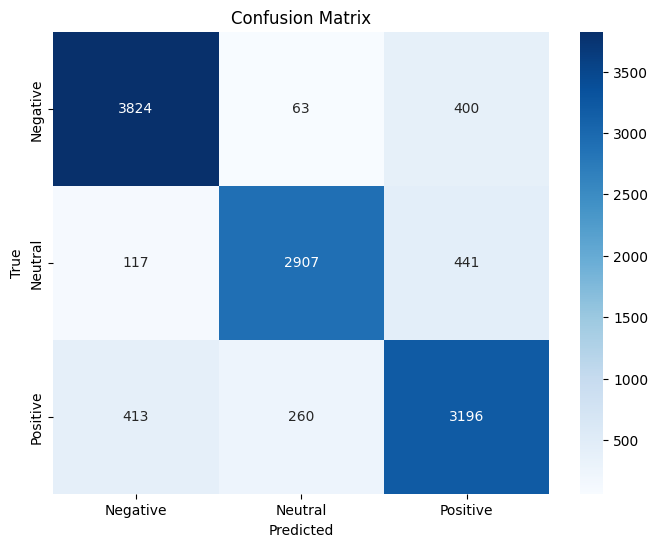
\includegraphics[width=\textwidth]{./images/cnn-cm.png}
\caption{CNN Architecture 2: CNN Confusion Matrix}
\label{fig:cnn2_loss}
\end{subfigure}
\caption{Training and Validation Performance of CNN Architecture 2}
\label{fig:cnn2_performance}
\end{figure}

This multi-filter CNN architecture showed significantly improved performance compared to the first CNN and the FNN models. It achieved a notably higher accuracy on the validation set, indicating better generalization capabilities due to its ability to extract diverse local patterns.

\begin{table}[H]
\centering
\caption{Classification Report for CNN Architecture 2 (Test Set)}
\begin{tabular}{|l|c|c|c|c|}
\hline
\textbf{Class} & \textbf{Precision} & \textbf{Recall} & \textbf{F1-Score} & \textbf{Support} \\
\hline
negative & 0.88 & 0.89 & 0.89 & 4287 \\
neutral  & 0.90 & 0.84 & 0.87 & 3465 \\
positive & 0.79 & 0.83 & 0.81 & 3869 \\
\hline
\textbf{Accuracy} & \multicolumn{4}{|c|}{\textbf{0.85}} \\
\hline
\end{tabular}
\label{tab:cnn2_classification_report}
\end{table}

This model achieved an accuracy of 0.85, demonstrating its effectiveness. The high precision and recall for 'negative' and 'neutral' classes are particularly good, though 'positive' sentiment shows a slightly lower precision.

However, even with these improvements, the training curves still indicate a slight degree of overfitting, Fig. \ref{fig:cnn2_loss}. While less pronounced than in the FNNs or the first CNN, the validation loss might still begin to rise slightly, or the validation accuracy might plateau while training accuracy continues to improve. This suggests that while the architecture is better suited for text, further regularization or more complex models might yield even better generalization.

Despite this minor overfitting, the second CNN architecture stands as a strong performer, achieving comparable results to our best SVM model and demonstrating the potential of CNNs for text classification tasks. Next we explore Recurrent Neural Networks to capture sequential dependencies in text.


\subsubsection{\textbf{Recurrent Neural Networks (RNNs)}}

Moving beyond models that primarily capture local features (like CNNs) or disregard sequence entirely (like FNNs), we implemented Recurrent Neural Networks (RNNs). RNNs are specifically designed to process sequential data, making them ideal for text. They maintain an internal state that allows them to remember information from previous steps in the sequence, which is crucial for understanding context and dependencies in sentences. We focused on two prominent RNN architectures: Long Short-Term Memory (LSTM) and Gated Recurrent Units (GRU).

\textbf{First LSTM Architecture: Simple LSTM}

Our initial RNN experiment utilized a basic Long Short-Term Memory (LSTM) layer. LSTMs are a type of RNN capable of learning long-term dependencies, addressing the vanishing gradient problem inherent in simpler RNNs.

The model's architecture is as follows:

\begin{itemize}
    \item Embedding Layer: Maps vocabulary words to 64-dimensional dense vectors, with maxlen input length.
    \item LSTM Layer (64 units): The core LSTM layer processing the sequence.
    \item Output Layer (3 units): Dense layer with Softmax activation for multiclass classification.
\end{itemize}

The model was compiled using categorical crossentropy loss and the Adam optimizer.

\begin{figure}[h!]
    \centering
    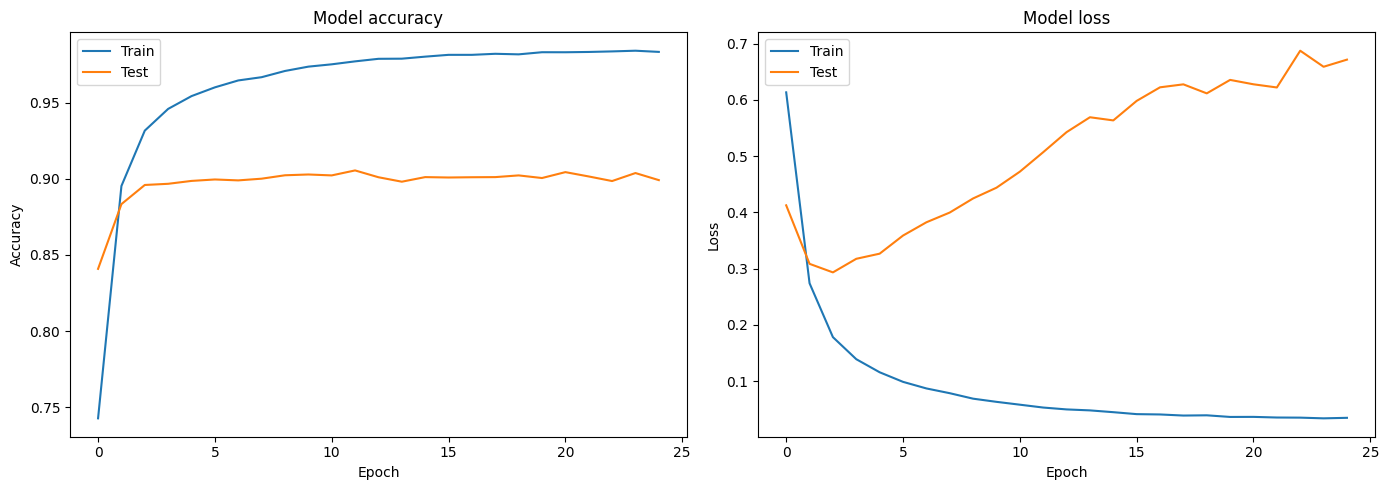
\includegraphics[width=1\linewidth]{images/lstm1.png}
    \caption{Simple LSTM Architecture: Train vs Validation Accuracy and Loss}
    \label{fig:enter-label}
\end{figure}

This basic LSTM model, despite its capability for sequential data, exhibited significant overfitting. While it learned to perform very well on the training data, its performance on the validation set quickly plateaued or even deteriorated. This suggests that the simple architecture lacked sufficient regularization or complexity to generalize effectively to unseen text.

\textbf{Second LSTM Architecture}

To combat the overfitting observed in the simple LSTM and further enhance performance, we developed a more complex LSTM architecture incorporating several regularization techniques.

The model's architecture is as follows:
\begin{itemize}
    \item Input Layer: Defines the input sequence shape (maxlen).
    \item Embedding Layer: Maps vocabulary words to a higher dimension (D=128), with mask\_zero=True to correctly handle padding.
    \item SpatialDropout1D Layer (0.8): Applies dropout to the entire feature map of the embedding, promoting independence between features.
    \item LSTM Layer (64 units): Processes the sequence, with dropout=0.3, recurrent\_dropout=0.3 (for regularization within the recurrent connections), return\_sequences=True (to pass output to the next layer if stacked LSTMs were used, though here it feeds into GlobalMaxPooling), and kernel\_regularizer=l2(0.01).
    \item GlobalMaxPooling1D Layer: Extracts the most salient feature from the LSTM output sequence.
    \item Dense Layer (64 units): Fully connected layer with ReLU activation and L2 regularization (0.001).
    \item BatchNormalization Layer: Normalizes activations.
    \item Dropout Layer (0.5): Regularization.
    \item Dense Layer (32 units): Another fully connected layer with ReLU activation.
    \item BatchNormalization Layer: Normalizes activations.
    \item Dropout Layer (0.5): Regularization.
    \item Output Layer (3 units): Dense layer with Softmax activation.
\end{itemize}

The model was compiled using the Adam optimizer with a learning rate of 0.001, categorical crossentropy loss.

\begin{figure}[h!]
\centering
\begin{subfigure}[t]{0.48\textwidth}
\centering
% Replace with your actual CNN 2 Accuracy plot
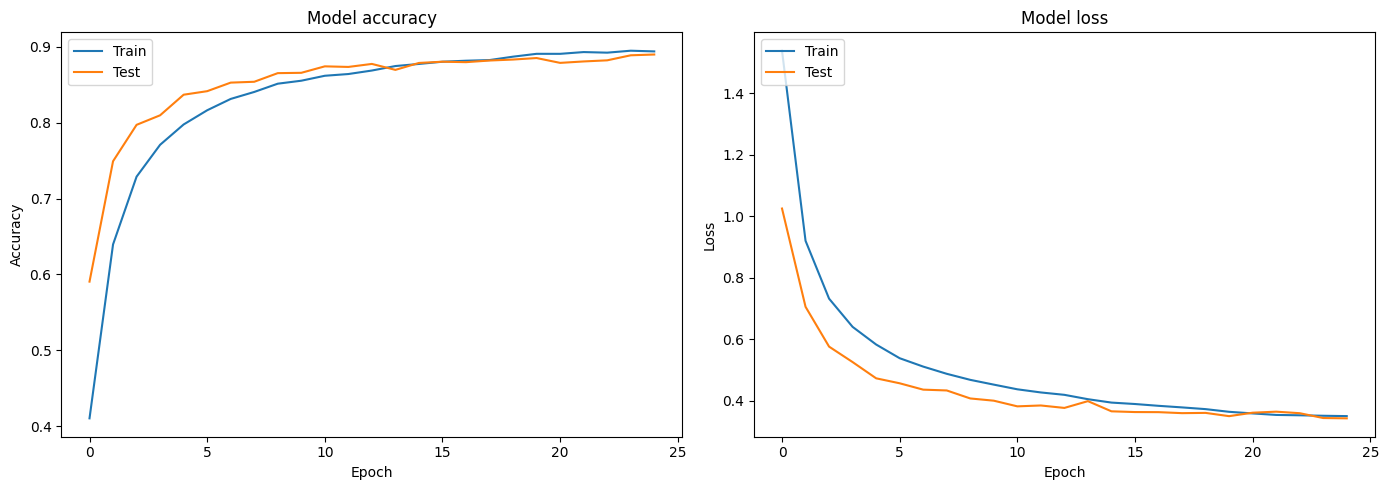
\includegraphics[width=\textwidth]{./images/lstm-acc.png}
\caption{LSTM Architecture 2: Train vs Validation Accuracy and Loss}
\label{fig:cnn2_ac1curacy}
\end{subfigure}
\hfill
\begin{subfigure}[t]{0.30\textwidth}
\centering
% Replace with your actual CNN 2 Loss plot
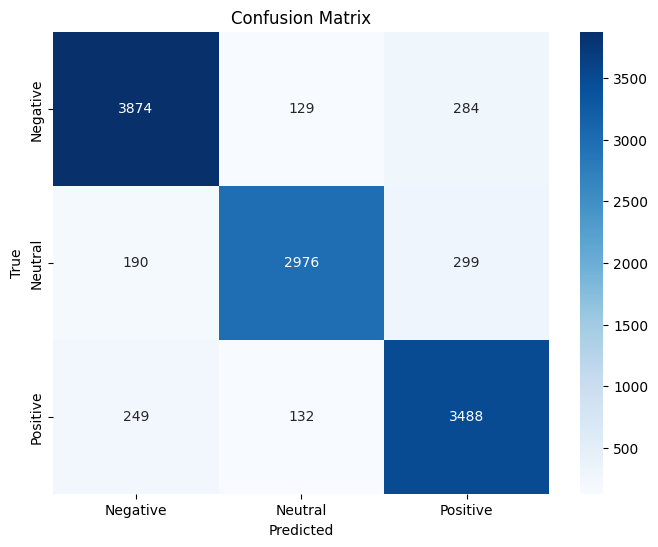
\includegraphics[width=\textwidth]{./images/lstm-cm.png}
\caption{LSTM Architecture 2: Confusion Matrix}
\label{fig:cnn2_lo1ss}
\end{subfigure}
\caption{Training and Validation Performance of LSTM Architecture 2}
\label{fig:cnn2_pe1rformance}
\end{figure}

This improved LSTM architecture demonstrated excellent performance on the test set, achieving a high accuracy and well-balanced precision, recall, and F1-scores across all sentiment classes. The various regularization techniques (SpatialDropout, recurrent dropout, L2 regularization, BatchNormalization, and Dropout) significantly reduced overfitting, leading to much better generalization.

\begin{table}[H]
\centering
\caption{Classification Report for Improved LSTM (Test Set)}
\begin{tabular}{|l|c|c|c|c|}
\hline
\textbf{Class} & \textbf{Precision} & \textbf{Recall} & \textbf{F1-Score} & \textbf{Support} \\
\hline
negative & 0.90 & 0.90 & 0.90 & 4287 \\
neutral  & 0.92 & 0.86 & 0.89 & 3465 \\
positive & 0.86 & 0.90 & 0.88 & 3869 \\
\hline
\textbf{Accuracy} & \multicolumn{4}{|c|}{\textbf{0.89}} \\
\hline
\end{tabular}
\label{tab:lstm2_classification_report}
\end{table}

This LSTM model achieved a remarkable overall accuracy of 0.89, marking it as one of the best-performing models thus far. Its ability to correctly classify 'neutral' tweets with high precision is particularly noteworthy.

\textbf{GRU Architecture: Gated Recurrent Unit
}

In parallel to the improved LSTM, we also developed a model based on Gated Recurrent Units (GRUs). GRUs are a slightly simplified variant of LSTMs, often offering comparable performance with fewer parameters, which can lead to faster training. Like LSTMs, they are designed to handle sequential data and mitigate the vanishing gradient problem.

The GRU model's architecture closely mirrors that of the improved LSTM, incorporating similar regularization strategies:

\begin{itemize}
    \item Input Layer: Defines the input sequence shape (maxlen).
    \item Embedding Layer: Maps vocabulary words to a higher dimension (D=128), with mask\_zero=True.
    \item SpatialDropout1D Layer (0.8): Applies dropout to the embedding feature map.
    \item GRU Layer (64 units): Processes the sequence, with dropout=0.3, recurrent\_dropout=0.3, return\_sequences=True, and kernel\_regularizer=l2(0.01).
    \item GlobalMaxPooling1D Layer: Extracts the most salient feature from the GRU output.
    \item Dense Layer (64 units): Fully connected layer with ReLU activation and L2 regularization (0.001).
    \item BatchNormalization Layer: Normalizes activations.
    \item Dropout Layer (0.5): Regularization.
    \item Dense Layer (32 units): Another fully connected layer with ReLU activation.
    \item BatchNormalization Layer: Normalizes activations.
    \item Dropout Layer (0.5): Regularization.
    \item Output Layer (3 units): Dense layer with Softmax activation.
\end{itemize}

The model was compiled using the Adam optimizer with a learning rate of 0.001, categorical crossentropy loss.

\begin{figure}[h!]
\centering
\begin{subfigure}[t]{0.48\textwidth}
\centering
% Replace with your actual CNN 2 Accuracy plot
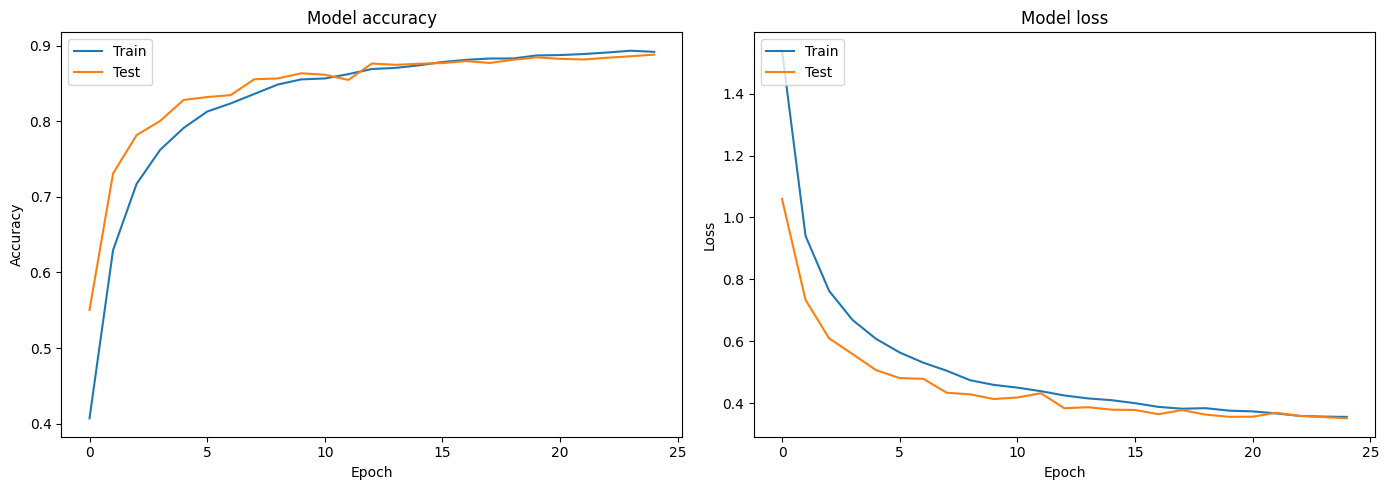
\includegraphics[width=\textwidth]{./images/gru-acc.png}
\caption{GRU Architecture: Train vs Validation Accuracy and Loss}
\label{fig:cnn22_accuracy}
\end{subfigure}
\hfill
\begin{subfigure}[t]{0.30\textwidth}
\centering
% Replace with your actual CNN 2 Loss plot
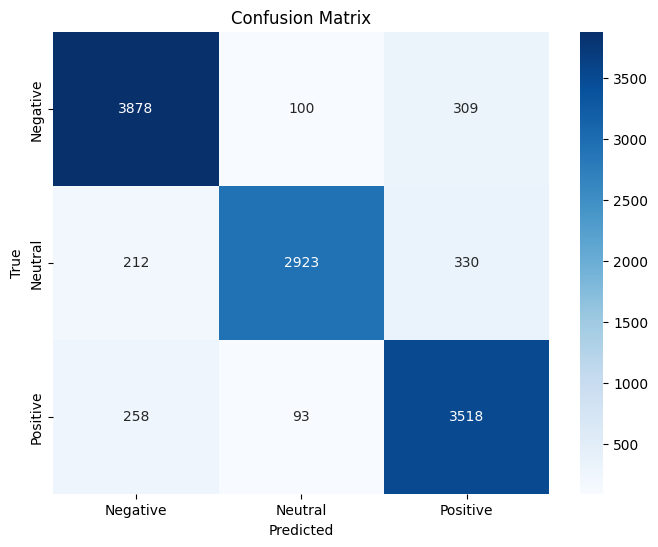
\includegraphics[width=\textwidth]{./images/gru-cm.png}
\caption{GRU Architecture: Confusion Matrix}
\label{fig:cnn24_loss}
\end{subfigure}
\caption{Training and Validation Performance of GRU Architecture}
\label{fig:cnn22_performance}
\end{figure}

The GRU model also yielded strong results on the test set, achieving an accuracy comparable to the improved LSTM. It demonstrated excellent precision and recall across all classes, showcasing its effectiveness in capturing sequential dependencies for sentiment analysis.

\begin{table}[H]
\centering
\caption{Classification Report for GRU Model (Test Set)}
\begin{tabular}{|l|c|c|c|c|}
\hline
\textbf{Class} & \textbf{Precision} & \textbf{Recall} & \textbf{F1-Score} & \textbf{Support} \\
\hline
negative & 0.89 & 0.90 & 0.90 & 4287 \\
neutral  & 0.94 & 0.84 & 0.89 & 3465 \\
positive & 0.85 & 0.91 & 0.88 & 3869 \\
\hline
\textbf{Accuracy} & \multicolumn{4}{|c|}{\textbf{0.89}} \\

\hline
\end{tabular}
\label{tab:gru_classification_report}
\end{table}

The GRU model achieved an overall accuracy of 0.89, matching the performance of the improved LSTM. It shows particularly high precision for the 'neutral' class and strong recall for 'negative' and 'positive' sentiments.

The similar high accuracy and balanced F1-scores between the improved LSTM and GRU models indicate that both architectures, when properly regularized and configured, are highly effective for sequential text classification tasks. Their ability to handle long-term dependencies and capture contextual information makes them superior to FNNs for this type of data, and their performance is on par with the best CNN model.

\textbf{Bidirectional LSTM (Bi-LSTM)}

In addition to the standard LSTM and GRU architectures, we also explored Bidirectional LSTMs (Bi-LSTMs). Bi-LSTMs enhance the ability of recurrent networks to understand context by processing the input sequence in both forward and backward directions independently, and then concatenating their outputs. This allows the model to capture dependencies from both past and future contexts, which can be particularly beneficial for tasks like sentiment analysis where the meaning of a word can be influenced by words that appear later in the sentence.

\begin{figure}[h!]
\centering
\begin{subfigure}[t]{0.48\textwidth}
\centering
% Replace with your actual CNN 2 Accuracy plot
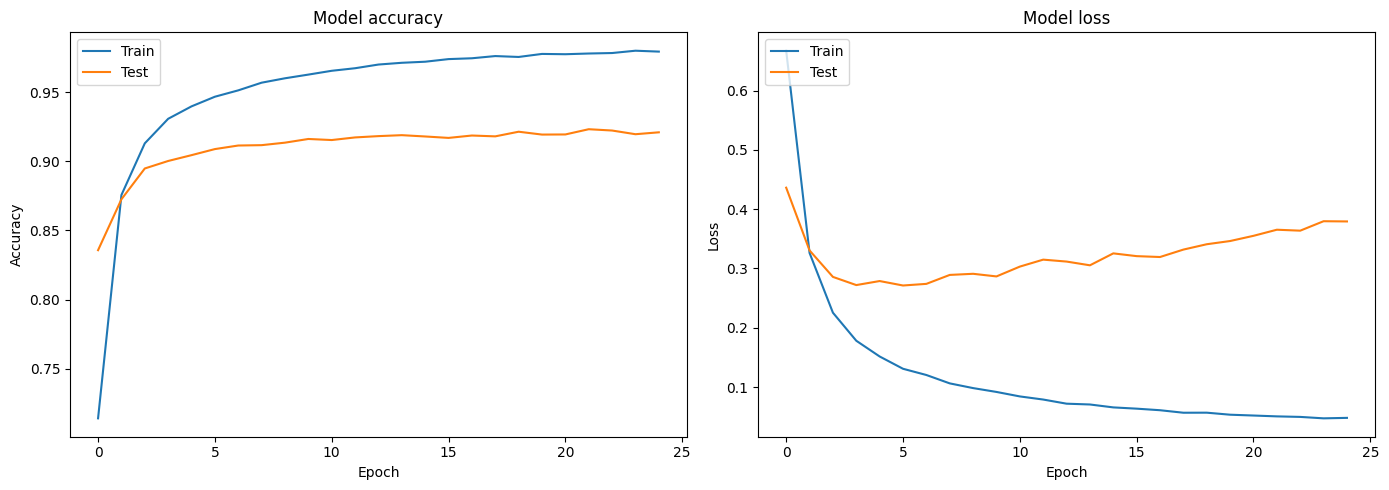
\includegraphics[width=\textwidth]{./images/bi1.png}
\caption{Bi-LSTM Architecture 1: Train vs Validation Accuracy and Loss}
\label{fig:cnn2_ac12curacy}
\end{subfigure}
\hfill
\begin{subfigure}[t]{0.48\textwidth}
\centering
% Replace with your actual CNN 2 Loss plot
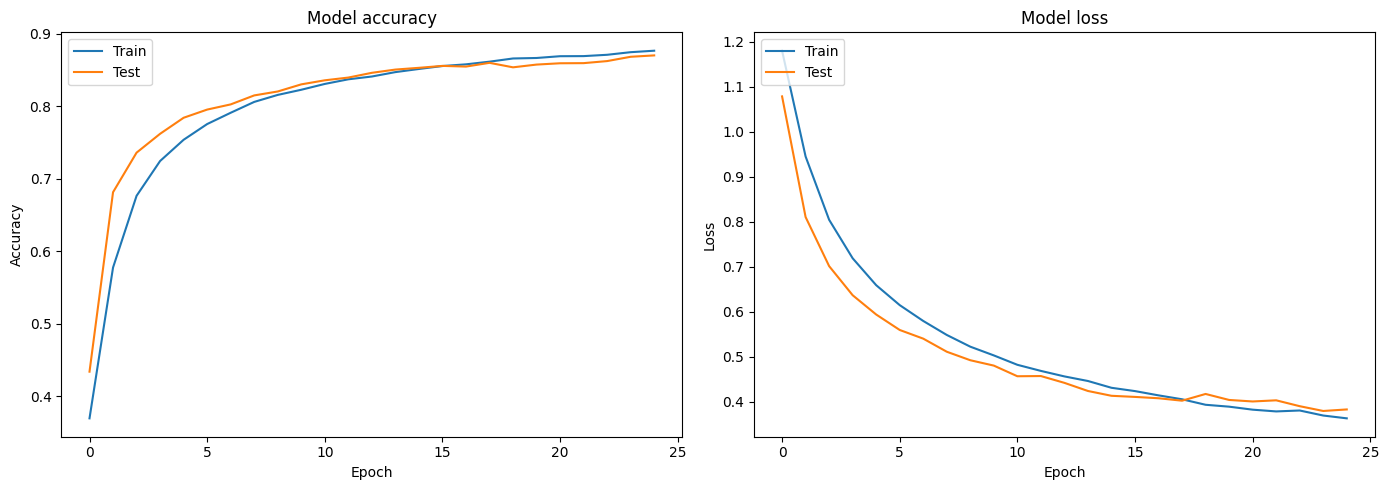
\includegraphics[width=\textwidth]{./images/bi2.png}
\caption{Bi-LSTM Architecture 2: Train vs Validation Accuracy and Loss}
\label{fig:cnn2_lo23ss}
\end{subfigure}
\caption{Training and Validation Performance of Bi-LSTM Architecture}
\label{fig:cnn2_2performance}
\end{figure}
\begin{table}[H]
\centering
\caption{Classification Report for Bi-LSTM Architecture 2 (Test Set)}
\begin{tabular}{|l|c|c|c|c|}
\hline
\textbf{Class} & \textbf{Precision} & \textbf{Recall} & \textbf{F1-Score} & \textbf{Support} \\
\hline
negative & 0.85 & 0.91 & 0.88 & 4285 \\
neutral  & 0.93 & 0.81 & 0.86 & 3507 \\
positive & 0.85 & 0.88 & 0.87 & 3829 \\
\hline
\textbf{Accuracy} & \multicolumn{4}{|c|}{\textbf{0.87}} \\
\hline
\end{tabular}
\label{tab:classification_report_modelo}
\end{table}

Similar to our other recurrent network experiments, our initial simple Bi-LSTM model exhibited significant overfitting, indicating that a basic configuration was insufficient to generalize effectively to unseen data. However, through the implementation of a second, more advanced Bi-LSTM architecture incorporating similar regularization techniques (such as SpatialDropout1D, recurrent dropout, and L2 regularization) as our improved LSTM and GRU models, we achieved similarly strong results. This improved Bi-LSTM model demonstrated excellent performance, effectively capturing the sequential nuances of the social media text and yielding high accuracy and well-balanced precision, recall, and F1-scores across all sentiment classes, aligning closely with the high-performing improved LSTM and GRU models.

\subsection{Transformer-based Models: BERT}

Finally, we tried into Transformer-based models, specifically BERT (Bidirectional Encoder Representations from Transformers). BERT models revolutionized Natural Language Processing (NLP) by pre-training deep bidirectional representations from unlabeled text, enabling them to understand context from both left and right sides of a word. This pre-training on massive datasets allows them to capture highly sophisticated linguistic patterns, making them incredibly powerful for various downstream tasks like sentiment analysis, typically through a process called fine-tuning.

\subsubsection{\textbf{Pre-trained BERT Model (cardiffnlp/twitter-roberta-base-sentiment)}}

Our initial approach involved directly utilizing a pre-trained BERT model specifically fine-tuned for sentiment analysis on Twitter data: cardiffnlp/twitter-roberta-base-sentiment \cite{camacho-collados-etal-2022-tweetnlp}. This model, a RoBERTa variant, is already optimized for social media text characteristics. We loaded its tokenizer and the pre-trained classification model and evaluated its performance on our dataset.

\begin{table}[H]
\centering
\caption{Classification Report for Pre-trained BERT (cardiffnlp/twitter-roberta-base-sentiment)}
\begin{tabular}{|l|c|c|c|c|}
\hline
\textbf{Class} & \textbf{Precision} & \textbf{Recall} & \textbf{F1-Score} & \textbf{Support} \\
\hline
negative & 0.68 & 0.76 & 0.72 & 21432 \\
neutral & 0.49 & 0.40 & 0.44 & 17327 \\
positive & 0.66 & 0.69 & 0.67 & 19342 \\
\hline
\textbf{Accuracy} & \multicolumn{4}{|c|}{\textbf{0.63}} \\
\hline
\end{tabular}
\label{tab:pretrained_bert_report}
\end{table}

While this pre-trained model provided a baseline, its overall accuracy of 0.6286 was not as high as anticipated, especially when compared to our better-performing CNN and RNN models. The F1-score for the 'neutral' class was particularly low, indicating that while it was trained on Twitter data, it might not perfectly align with the specific distribution or nuances of sentiment in our dataset. This suggested that a custom fine-tuning approach would be more beneficial.



\subsubsection{\textbf{BERT Fine-tuning for Sentiment Classification}}

Given the limitations of the directly applied pre-trained model, we proceeded with fine-tuning a BERT model on our specific dataset. Fine-tuning involves continuing the training of a pre-trained model on a smaller, task-specific dataset, allowing it to adapt its learned representations to the new task while retaining its general language understanding.

The fine-tuned BERT model achieved superior results compared to all previous models, demonstrating the power of transfer learning from large-scale pre-trained transformers.

\begin{table}[H]
\centering
\caption{Classification Report for Fine-tuned BERT (Test Set)}
\begin{tabular}{|l|c|c|c|c|}
\hline
\textbf{Class} & \textbf{Precision} & \textbf{Recall} & \textbf{F1-Score} & \textbf{Support} \\
\hline
negative & 0.92 & 0.93 & 0.93 & 4287 \\
neutral  & 0.93 & 0.92 & 0.92 & 3465 \\
positive & 0.92 & 0.92 & 0.92 & 3869 \\
\hline
\textbf{Accuracy} & \multicolumn{4}{|c|}{\textbf{0.93}} \\
\hline
\end{tabular}
\label{tab:fine_tuned_bert_report}
\end{table}

The fine-tuned BERT model achieved an impressive overall accuracy of 0.93, making it the highest-performing model in our entire evaluation. It demonstrated consistently high precision, recall, and F1-scores across all three sentiment classes, indicating robust and balanced classification performance.

\begin{figure}[h!]
\centering
\begin{subfigure}[t]{0.48\textwidth}
\centering
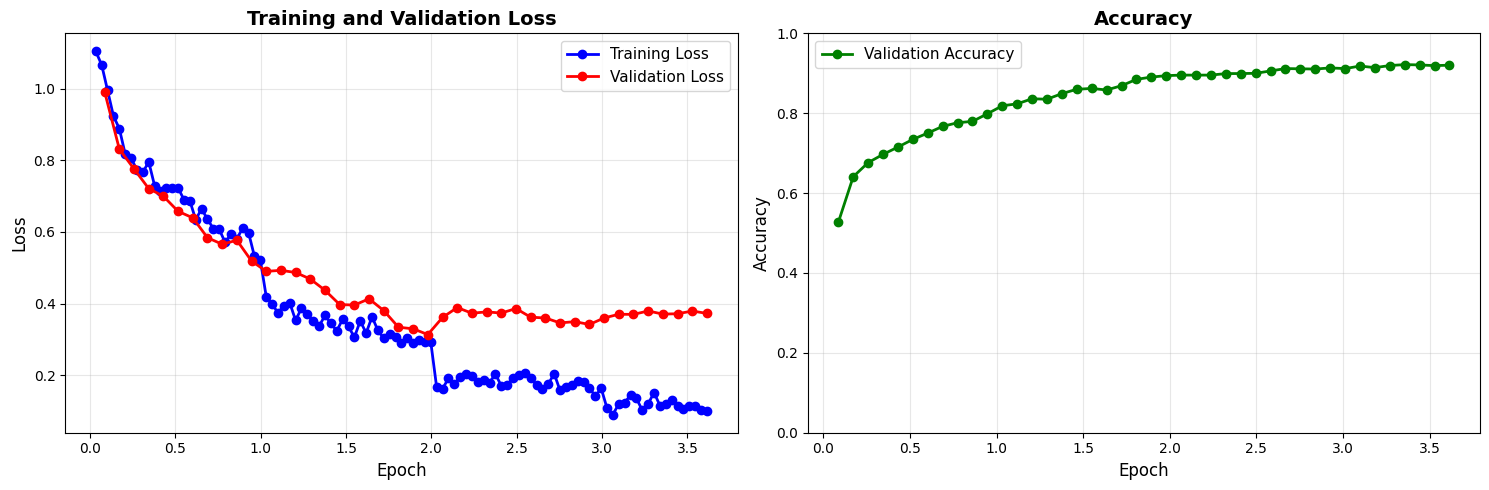
\includegraphics[width=\textwidth]{./images/bert.png}
\caption{Fine-tuned BERT: Training and Validation Loss and Accuracy}
\label{fig:bert_loss}
\end{subfigure}
\hfill
\begin{subfigure}[t]{0.48\textwidth}
\centering
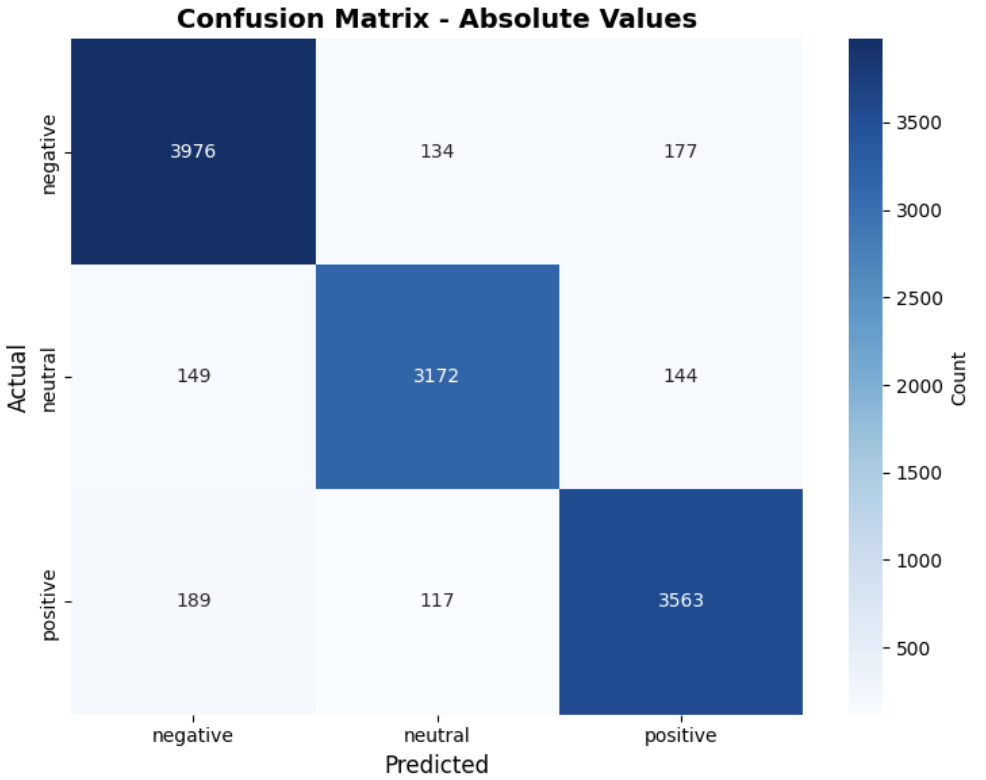
\includegraphics[width=0.4\textwidth]{./images/bert-cm.png}
\caption{Fine-tuned BERT: Confusion Matrix}
\label{fig:bert_accuracy}
\end{subfigure}
\caption{Training and Validation Performance of Fine-tuned BERT Model}
\label{fig:bert_performance}
\end{figure}

The per-class analysis also highlights the model's balanced performance:
\begin{itemize}
\item Negative: Accuracy=0.93, Count=4287
\item Neutral: Accuracy=0.92, Count=3465
\item Positive: Accuracy=0.92, Count=3869
\end{itemize}

\subsubsection{\textbf{Computational Considerations}}

It is important to note that while BERT models deliver state-of-the-art performance, they are significantly more computationally intensive than the traditional machine learning models (SVMs) and even the simpler deep learning architectures (FNNs, CNNs, RNNs). Training the BERT model, even with fine-tuning, required substantial computational resources and took approximately 4 to 5 hours to complete on our setup. This computational cost is a crucial factor to consider when deploying such models, especially in resource-constrained environments or for real-time applications.

Despite the higher computational demands, the fine-tuned BERT model consistently yielded the best performance across all experiments, affirming its position as a leading approach for complex NLP tasks like sentiment analysis on social media text. Our further experiments with various parameters consistently confirmed BERT's superior results.







